\documentclass[a4paper, 12pt]{article}

\usepackage[french]{babel} 
\usepackage[utf8]{inputenc}
\usepackage[T1]{fontenc} 
\usepackage{amsmath}
\usepackage{amssymb}
\usepackage{listings}  
\usepackage{graphicx}
\usepackage[margin=2.5cm]{geometry}
\usepackage{amsmath,amsfonts,amssymb}
\usepackage{hyperref}
\lstset{
language=Java,
breaklines=true
}



\newcommand*{\plogo}{\fbox{$\mathcal{PL}$}} % Generic publisher logo

%----------------------------------------------------------------------------------------
%	TITLE PAGE
%----------------------------------------------------------------------------------------

\newcommand*{\titleGM}{\begingroup % Create the command for including the title page in the document
\hbox{ % Horizontal box
\hspace*{0.2\textwidth} % Whitespace to the left of the title page
\rule{2pt}{\textheight} % Vertical line
\hspace*{0.05\textwidth} % Whitespace between the vertical line and title page text
\parbox[b]{0.75\textwidth}{ % Paragraph box which restricts text to less than the width of the page

{\noindent\Huge\bfseries Software Project\\ Engineering }\\[2\baselineskip] % Title
{\Large \textit{Phase 1 Report}}\\[4\baselineskip] % Tagline or further description
{\Large \textbf{Project leader} : Hélène Verhaeghe}
\\
{\Large \textsc{\textbf{Group E}}\\\textsc{Aurian De Potter(Group leader)},\\ \textsc{Eddy Ndizera},\\ \textsc{Ivan Ahad},\\ \textsc{Arnaud Dethise},\\ \textsc{Ludovic Fastré},\\ \textsc{Anthony Dechamps},\\ \textsc{Geoffroy Husson},\\ \textsc{Jonathan Legat}} % Author name

\vspace{0.5\textheight} % Whitespace between the title block and the publisher
{\noindent \Large \textbf{INGI2255}}\\[\baselineskip] % Publisher and logo
}\\

}
\endgroup}


\clearpage
\setcounter{page}{0}
\begin{document}
\titleGM
\section{Introduction}
After all the requirements were set in the launching report, we started developing the ones we had planned to implement for the first sprint. We will explain in the report which of them have been implemented, we will also talk about a change in the tools we are using, and we will show a couple of diagrams of our software. Please note that we decided not to make the mockups yet for this phase, as we will make them in a future one. 

\section{Important change}

The group decided to change the Control Version System used, switching from \textbf{mercurial} to \textbf{git}. This was decided because it was more convenient as all the members already had a good experience with git and were used to it. Moreover, when it comes to managing merging collisions, git has a user-friendly way of dealing with them. We also decided to use GitHub instead of BitBucket. The advantage of BitBucket is that it has a private repository and manages mercurial. However, this requires us to have accounts with the student pack. Some members did have the pack so GitHub had all the advantages that BitBucket offered to us. But as we are not using mercurial anymore, we are more than satisfied with GitHub, because if the clients wish to publish the source code, then it is more interesting to use GitHub due to the fact that we can switch the repository to public mode and its community is much larger.

\section{Requirements developed in this phase}

	The requirements below are the ones we planned to develop during the first phase. No change occurred during the phase and we are happy to have completed the requirements we said we would do(\textit{See explanation about this later}). We have implemented what we considered to be the base of the project so that we have something to start with. This consists of the creation of the different pages needed to register a player, a court and the staff and admin pages. The database was also created with the different tables for the user, the staff, etc. We have chosen a template design that is subject to change all along the project. Plus, a host was created as advised during our last appointment. The link is \url{https://sep2015e.herokuapp.com}.\\ 
	
\begin{itemize}
\item The user can register as a pair to a tournament by filling in the form.
\item The user can register for activities during a tournament (barbecue, etc) and choose preferences such as taking responsibilities and payment method
\item Common page for staff members
\item The system can create pools and match ups
\item After a pool has been generated, a staff member can manually reorganize it : \textit{We actually decided to not implement this feature as we actually thought it was not necessary, at least for this phase. We might still implement it if the client do think it is necessary}
\item An admin can close the registration for a tournament (and trigger the creation of pools) \\

\end{itemize}

It is important to note that this list does not show the order in which we implemented all the feature. As we said in the previous report, we used \textit{Trello} to divide the work between our group. Each member focused on one requirement at a time  specifically, and we sometimes worked in pairs for some of them. Also, this was more of a warm-up phase so each member has now learned how others work. If you are interested in seeing the work accomplished by each member, we can invite you into our Trello and Github but we will still briefly present how the work was distributed among the group. \\

Aurian, Anthony and Jonathan took care of the forms of the registration of pairs and for the registration of activies. Geoffroy and Eddy implemented the page that is going to be used by staff accounts. Arnaud and Ivan implemented the system that allows to create pools and matchup, and also the feature that allows an admin to close the registration for a tournament. Finally, Ludovic took care of most of the design of the software, and worked on the administration system.
\section{ORM diagram}

 Fig.\ref{ORM_diagram} shows our ORM diagram. It gives an idea about how the different objects used by the website are linked together. We will give a brief description of what the object represents and its relations to others. We will ask you to zoom in the PDF file, as it was a challenge to make the diagrams fit completely in the report, we apologize for the inconvenience.\\
 
 The \textit{user} represents a player participating in the tournament. It is characterized by a name, an email, an address and the level of the player (meaning how good he is at tennis). \\
 
 A \textit{pair} is formed of two users. A single pair can only participate in one \textit{pool} of the \textit{tournament}. A pool contains pairs and their \textit{match} (matchups between pairs). A match is characterized by the pairs confronting each other and the \textit{court} in which they will play. The court object contains information about the court owner, the address of it and finally some comments about it like the type of surface. \\
 
 As we said, a tournament is composed of pools but also of a knock-off tournament that we called \textit{tree} in our diagram. Moreover, a tournament is defined by its \textit{category}. Finally, the tree is composed of \textit{nodes} that is basically a pair of two users. \\
 
 This concludes the description about the ORM diagram. We still must inform you the diagram may change. We may add more objects or change the links between them. But we will take care as to write out the changes done in case we modify it.
 
\begin{figure}
	\caption{ORM diagram}
	\label{ORM_diagram}
	\includegraphics[scale=0.5, angle=270]{ORMfinal.png}

\end{figure}

\newpage
\section{Architecture of the software and UML Diagram}
We can see in Fig.\ref{UML_diagram} our class diagram, describing the architecture of our software. We mostly followed the regular architecture offered by Django. The diagram was structured by the packages and the ".py" files, for example "players(package).models(.py).User". Some files only contain methods but it was still important to put them in the diagram. 
\\

The class diagram contains 4 very important parts. One represents the players, the second is the staff, the third is the tournament and the fourth is the courts.\\

As you can guess, the players part contains all the functions for the savings of data about a player and those that allow him to register for the tournament.\\

The staff part is composed of the views to display the staff webpage. It also contains methods to allow staff members to send messages to each others.\\

The tournament contains all the methods needed to generate a tournament and close it (at the end of registration).\\

Lastly, the courts part allows a court owner to register himself and his court(s).\\

\noindent
\begin{figure}
	\caption{UML diagram}
	\label{UML_diagram}
	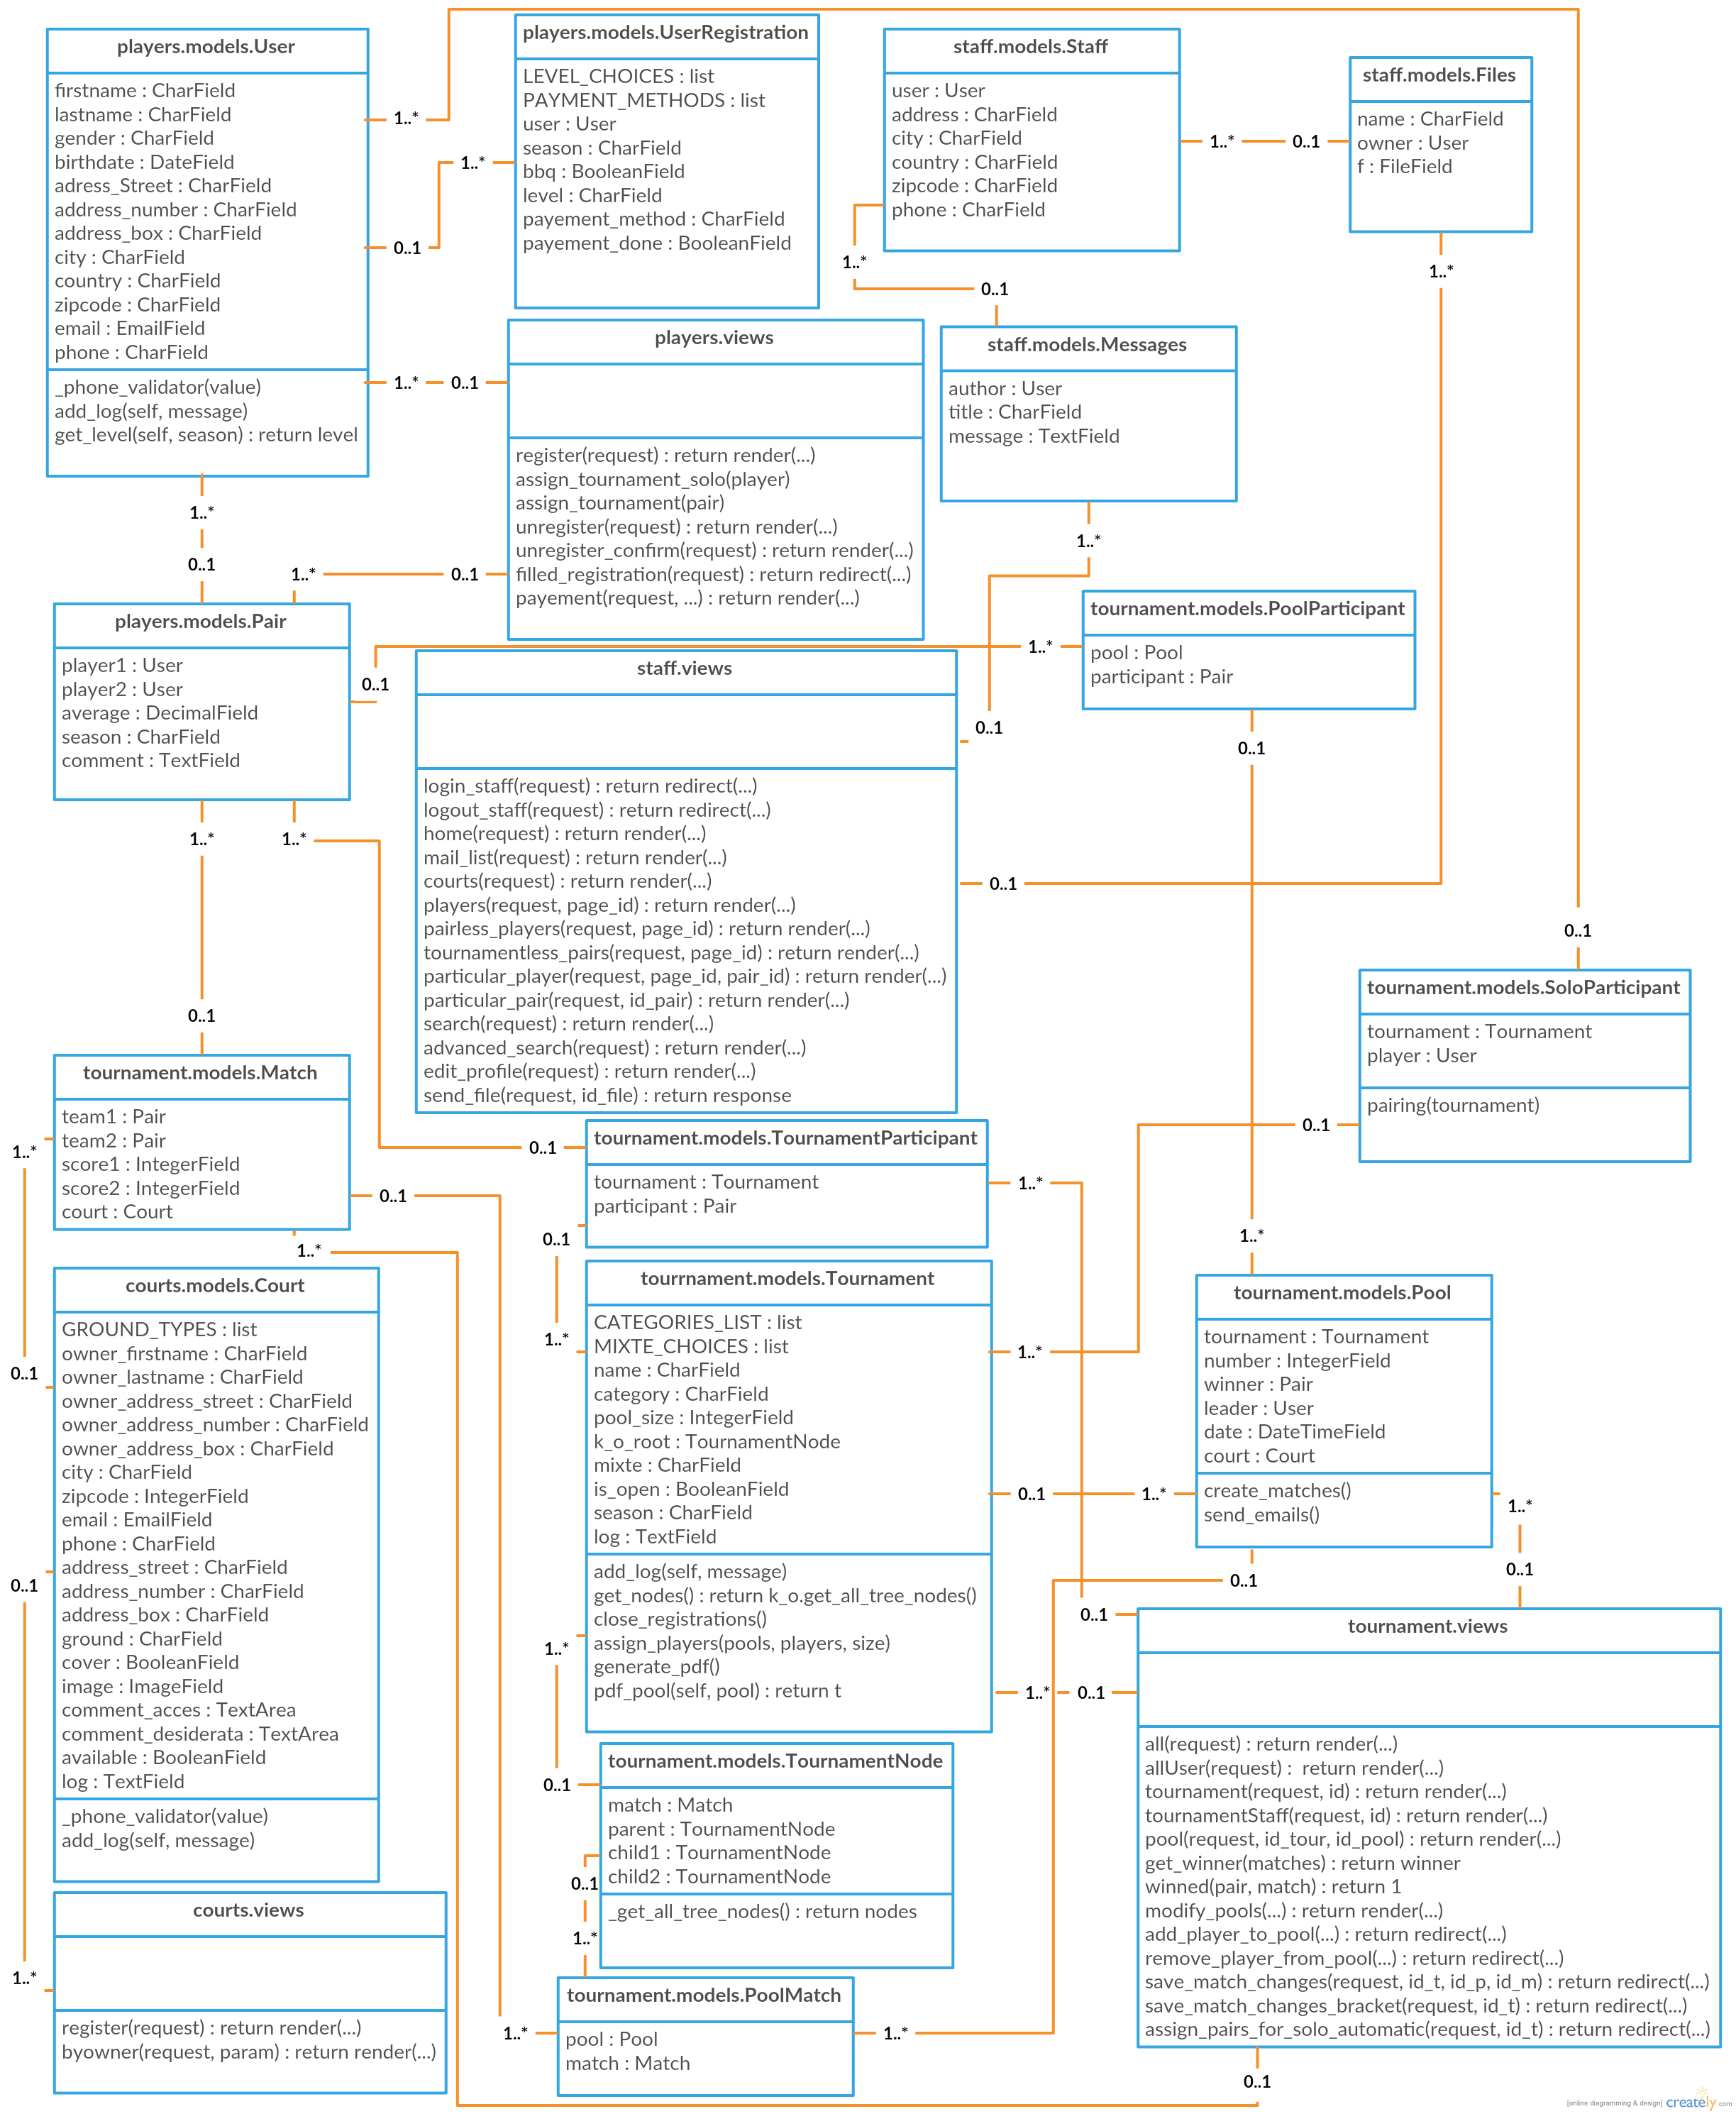
\includegraphics[width=18cm]{Class.png}

\end{figure}

\section{Conclusion}
As we have seen in the report, we have implemented the requirements that we thought were necessary to be developed for the first phase. According to the feedback session that we will have next week, we will see if the development is following the right direction, and we are going to work accordingly for the next phases. 

\end{document}